\documentclass[portrait]{seminar}
%\usepackage{pandora}
\usepackage{color}
\usepackage{fancybox}
\usepackage{alltt}
\usepackage{epsfig}
\usepackage{rail}
\usepackage{bar}
\usepackage{url}
\usepackage{rotating}
\usepackage[normalem]{ulem}
\usepackage{latexsym}
\usepackage{amsmath}

\begin{document}

\boldmath
\newcommand{\RA}{$\rightarrow$}
\newcommand{\LL}{\mbox{$[$\hspace{-0.15em}$[$}}
\newcommand{\RR}{\mbox{$]$\hspace{-0.15em}$]$}}
\newcommand{\CC}[1]{\mbox{\tt $\LL$#1$\RR$}}

\slideframe{shadow}

%%% Activate one of these to get either Aarhus style or McGill style 
%%% by putting a #1 in the appropriate line.
\newcommand{\mcgill}[1]{#1}
\newcommand{\aarhus}[1]{}

%%% Define this to be the name of your term
\newcommand{\courseterm}{Fall 2012}




\aarhus{
\newpagestyle{dOvsstyle}{dOvs \courseterm Week 37 \hfil Scanners and Parsers}{\hfil \thepage}
}

\mcgill{
\newpagestyle{dOvsstyle}{COMP 520 \courseterm  \hfil Scanners and Parsers (\thepage)}{}
}

\slidepagestyle{dOvsstyle}

\begin{slide*}
\begin{tabbing}
\aarhus{ {\Large\bf Week 37}\\}
~\\
{\Huge\bf Scanners and}\\ ~\\ {\Huge\bf parsers}\\
\end{tabbing}

\begin{center}
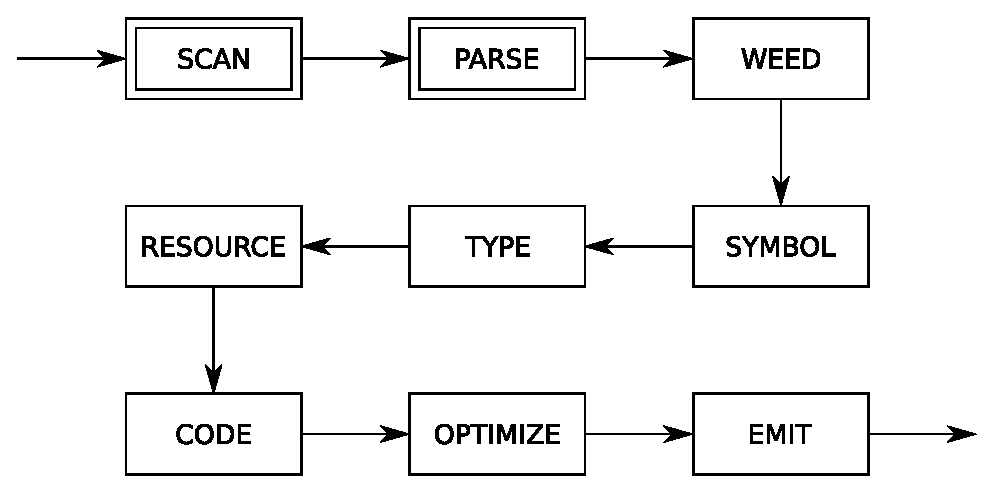
\psfig{file=figs/scan_parse.eps,width=20em}
\end{center}

\vfil
\end{slide*}

\begin{slide*}
A {\em scanner\/} or {\em lexer} transforms a string of characters into a string
of tokens:
\begin{itemize}
\item uses a combination of {\em deterministic finite automata} (DFA);
\item plus some glue code to make it work;
\item can be generated by tools like {\tt flex} (or {\tt lex}), {\tt JFlex}, \ldots 
\end{itemize}
\vspace*{1em}
\begin{center}
\setlength{\unitlength}{2300sp}%
%
\begingroup\makeatletter\ifx\SetFigFont\undefined%
\gdef\SetFigFont#1#2#3#4#5{%
  \reset@font\fontsize{#1}{#2pt}%
  \fontfamily{#3}\fontseries{#4}\fontshape{#5}%
  \selectfont}%
\fi\endgroup%
\begin{picture}(5424,5124)(1189,-6673)
\thicklines
\put(1801,-3361){\oval(1200,600)}
\put(3901,-4861){\oval(1200,600)}
\put(6001,-4861){\oval(1200,600)}
\put(1201,-2161){\framebox(1200,600){}}
\put(1201,-5161){\framebox(1200,600){}}
\put(5401,-3661){\framebox(1200,600){}}
\put(5401,-6661){\framebox(1200,600){}}
\put(1801,-2161){\vector( 0,-1){900}}
\put(1801,-3661){\vector( 0,-1){900}}
\put(2401,-4861){\vector( 1, 0){900}}
\put(4501,-4861){\vector( 1, 0){900}}
\put(6001,-3661){\vector( 0,-1){900}}
\put(6001,-5161){\vector( 0,-1){900}}
\put(1451,-1916){\makebox(0,0)[lb]{\smash{\SetFigFont{8}{14.4}{\ttdefault}{\mddefault}{\updefault}joos.l}}}
\put(1536,-3416){\makebox(0,0)[lb]{\smash{\SetFigFont{8}{14.4}{\ttdefault}{\mddefault}{\updefault}flex}}}
\put(1326,-4916){\makebox(0,0)[lb]{\smash{\SetFigFont{8}{14.4}{\ttdefault}{\mddefault}{\updefault}lex.yy.c}}}
\put(3701,-4916){\makebox(0,0)[lb]{\smash{\SetFigFont{8}{14.4}{\ttdefault}{\mddefault}{\updefault}gcc}}}
\put(5601,-4916){\makebox(0,0)[lb]{\smash{\SetFigFont{8}{14.4}{\ttdefault}{\mddefault}{\updefault}scanner}}}
\put(5551,-3416){\makebox(0,0)[lb]{\smash{\SetFigFont{8}{14.4}{\ttdefault}{\mddefault}{\updefault}foo.joos}}}
\put(5651,-6416){\makebox(0,0)[lb]{\smash{\SetFigFont{8}{14.4}{\ttdefault}{\mddefault}{\updefault}tokens}}}
\end{picture}
\end{center}

\vfil
\end{slide*}

\begin{slide*}
A {\em parser\/} transforms a string of tokens into a parse tree, according to some
grammar:
\begin{itemize}
\item it corresponds to a {\em deterministic push-down automaton};
\item plus some glue code to make it work;
\item can be generated by {\tt bison} (or {\tt yacc}), CUP, ANTLR, SableCC,
Beaver, JavaCC, \ldots
\end{itemize}
\vspace*{1em}
\begin{center}
\setlength{\unitlength}{2300sp}%
%
\begingroup\makeatletter\ifx\SetFigFont\undefined%
\gdef\SetFigFont#1#2#3#4#5{%
  \reset@font\fontsize{#1}{#2pt}%
  \fontfamily{#3}\fontseries{#4}\fontshape{#5}%
  \selectfont}%
\fi\endgroup%
\begin{picture}(5424,5124)(1189,-6673)
\thicklines
\put(1801,-3361){\oval(1200,600)}
\put(3901,-4861){\oval(1200,600)}
\put(6001,-4861){\oval(1200,600)}
\put(1201,-2161){\framebox(1200,600){}}
\put(1201,-5161){\framebox(1200,600){}}
\put(5401,-3661){\framebox(1200,600){}}
\put(5401,-6661){\framebox(1200,600){}}
\put(1801,-2161){\vector( 0,-1){900}}
\put(1801,-3661){\vector( 0,-1){900}}
\put(2401,-4861){\vector( 1, 0){900}}
\put(4501,-4861){\vector( 1, 0){900}}
\put(6001,-3661){\vector( 0,-1){900}}
\put(6001,-5161){\vector( 0,-1){900}}
\put(1451,-1916){\makebox(0,0)[lb]{\smash{\SetFigFont{8}{14.4}{\ttdefault}{\mddefault}{\updefault}joos.y}}}
\put(1506,-3416){\makebox(0,0)[lb]{\smash{\SetFigFont{8}{14.4}{\ttdefault}{\mddefault}{\updefault}bison}}}
\put(1356,-4916){\makebox(0,0)[lb]{\smash{\SetFigFont{8}{14.4}{\ttdefault}{\mddefault}{\updefault}y.tab.c}}}
\put(3701,-4916){\makebox(0,0)[lb]{\smash{\SetFigFont{8}{14.4}{\ttdefault}{\mddefault}{\updefault}gcc}}}
\put(5651,-4916){\makebox(0,0)[lb]{\smash{\SetFigFont{8}{14.4}{\ttdefault}{\mddefault}{\updefault}parser}}}
\put(5621,-3416){\makebox(0,0)[lb]{\smash{\SetFigFont{8}{14.4}{\ttdefault}{\mddefault}{\updefault}tokens}}}
\put(5821,-6416){\makebox(0,0)[lb]{\smash{\SetFigFont{8}{14.4}{\ttdefault}{\mddefault}{\updefault}AST}}}
\end{picture}
\end{center}

\vfil
\end{slide*}


\begin{slide*}
Tokens are defined by {\em regular expressions}:
\begin{itemize}
\item $\emptyset$, the empty set: a language with no strings
\item $\varepsilon$, the empty string
\item $a$, where $a \in \Sigma$ and $\Sigma$ is our alphabet
\item $M | N$, alternation: either $M$ or $N$
\item $M \cdot N$, concatenation: $M$ followed by $N$
\item $M^{*}$, zero or more occurences of $M$
\end{itemize}
where $M$ and $N$ are both regular expressions.  What are $M$? and $M^{+}$?

\vspace{.2in}

We can write regular expressions for the
tokens in our source language using standard POSIX notation: 
\begin{itemize}
\item simple operators: \verb:"*":, \verb:"/":, \verb:"+":, \verb:"-":
\item parentheses: \verb:"(":, \verb:")":
\item integer constants: \verb:0|([1-9][0-9]*):
\item identifiers: \verb:[a-zA-Z_][a-zA-Z0-9_]*:
\item white space: \verb*:[ \t\n]+:
\end{itemize}

\vfil
\end{slide*}

\begin{slide*}
{\tt flex} accepts a list of regular expressions (regex), converts each regex
internally to an NFA (Thompson construction), and then converts each NFA to a DFA (see Appel,
Ch. 2):
\vspace*{3em}

\setlength{\unitlength}{0.0004in}%
%
\begingroup\makeatletter\ifx\SetFigFont\undefined%
\gdef\SetFigFont#1#2#3#4#5{%
  \reset@font\fontsize{#1}{#2pt}%
  \fontfamily{#3}\fontseries{#4}\fontshape{#5}%
  \selectfont}%
\fi\endgroup%
\begin{picture}(7445,5570)(889,-7198)
\thicklines
\put(5401,-1861){\circle{450}}
\put(5401,-1861){\circle{300}}
\put(4201,-1861){\circle{450}}
\put(4426,-1861){\vector( 1, 0){750}}
\put(3601,-1861){\vector( 1, 0){375}}
\put(8101,-1861){\circle{450}}
\put(8101,-1861){\circle{300}}
\put(6901,-1861){\circle{450}}
\put(7126,-1861){\vector( 1, 0){750}}
\put(6301,-1861){\vector( 1, 0){375}}
\put(2701,-1861){\circle{450}}
\put(2701,-1861){\circle{300}}
\put(1501,-1861){\circle{450}}
\put(1726,-1861){\vector( 1, 0){750}}
\put(901,-1861){\vector( 1, 0){375}}
\put(5401,-3061){\circle{450}}
\put(5401,-3061){\circle{300}}
\put(4201,-3061){\circle{450}}
\put(4426,-3061){\vector( 1, 0){750}}
\put(3601,-3061){\vector( 1, 0){375}}
\put(8101,-3061){\circle{450}}
\put(8101,-3061){\circle{300}}
\put(6901,-3061){\circle{450}}
\put(7126,-3061){\vector( 1, 0){750}}
\put(6301,-3061){\vector( 1, 0){375}}
\put(2701,-3061){\circle{450}}
\put(2701,-3061){\circle{300}}
\put(2626,-4111){\circle{450}}
\put(2626,-4111){\circle{300}}
\put(2626,-5011){\circle{450}}
\put(2626,-5011){\circle{300}}
\put(6001,-4561){\circle{450}}
\put(6001,-4561){\circle{300}}
\put(2701,-6661){\circle{450}}
\put(2701,-6661){\circle{300}}
\put(1501,-6661){\circle{450}}
\put(2701,-6886){\line( 0,-1){300}}
\put(2701,-7186){\line( 1, 0){450}}
\put(3151,-7186){\line( 0, 1){1125}}
\put(3151,-6061){\line(-1, 0){450}}
\put(2701,-6061){\vector( 0,-1){375}}
\put(1726,-6661){\vector( 1, 0){750}}
\put(901,-6661){\vector( 1, 0){375}}
\put(1750,-6546){\makebox(0,0)[lb]{\smash{\SetFigFont{8}{14.4}{\ttdefault}{\mddefault}{\updefault}{\tt \symbol{32}\symbol{92}t\symbol{92}n}}}}
\put(3226,-6736){\makebox(0,0)[lb]{\smash{\SetFigFont{8}{14.4}{\ttdefault}{\mddefault}{\updefault}{\tt \symbol{32}\symbol{92}t\symbol{92}n}}}}
\put(1501,-3061){\circle{450}}
\put(1501,-4561){\circle{450}}
\put(4201,-4561){\circle{450}}
\put(1726,-3061){\vector( 1, 0){750}}
\put(901,-3061){\vector( 1, 0){375}}
\put(1726,-4561){\vector( 3, 2){675}}
\put(1726,-4561){\vector( 3,-2){675}}
\put(2626,-5236){\line( 0,-1){375}}
\put(2626,-5611){\line( 1, 0){450}}
\put(3076,-5611){\line( 0, 1){1200}}
\put(3076,-4411){\line(-1, 0){450}}
\put(2626,-4411){\vector( 0,-1){375}}
\put(901,-4561){\vector( 1, 0){375}}
\put(4426,-4561){\vector( 1, 0){1350}}
\put(6001,-4786){\line( 0,-1){375}}
\put(6001,-5161){\line( 1, 0){450}}
\put(6451,-5161){\line( 0, 1){1200}}
\put(6451,-3961){\line(-1, 0){450}}
\put(6001,-3961){\vector( 0,-1){375}}
\put(3601,-4561){\vector( 1, 0){375}}
\put(2026,-1786){\makebox(0,0)[lb]{\smash{\SetFigFont{8}{14.4}{\ttdefault}{\mddefault}{\updefault}*}}}
\put(4726,-1786){\makebox(0,0)[lb]{\smash{\SetFigFont{8}{14.4}{\ttdefault}{\mddefault}{\updefault}/}}}
\put(7426,-1786){\makebox(0,0)[lb]{\smash{\SetFigFont{8}{14.4}{\ttdefault}{\mddefault}{\updefault}+}}}
\put(4726,-2986){\makebox(0,0)[lb]{\smash{\SetFigFont{8}{14.4}{\ttdefault}{\mddefault}{\updefault}(}}}
\put(7501,-2986){\makebox(0,0)[lb]{\smash{\SetFigFont{8}{14.4}{\ttdefault}{\mddefault}{\updefault})}}}
\put(2026,-2986){\makebox(0,0)[lb]{\smash{\SetFigFont{8}{14.4}{\ttdefault}{\mddefault}{\updefault}-}}}
\put(1951,-4261){\makebox(0,0)[lb]{\smash{\SetFigFont{8}{14.4}{\ttdefault}{\mddefault}{\updefault}0}}}
\put(3151,-5086){\makebox(0,0)[lb]{\smash{\SetFigFont{8}{14.4}{\ttdefault}{\mddefault}{\updefault}0-9}}}
\put(1670,-5011){\makebox(0,0)[lb]{\smash{\SetFigFont{8}{14.4}{\ttdefault}{\mddefault}{\updefault}1-9}}}
\put(6526,-4636){\makebox(0,0)[lb]{\smash{\SetFigFont{8}{14.4}{\ttdefault}{\mddefault}{\updefault}a-zA-Z0-9\_}}}
\put(4631,-4446){\makebox(0,0)[lb]{\smash{\SetFigFont{8}{14.4}{\ttdefault}{\mddefault}{\updefault}a-zA-Z\_}}}
\end{picture}

~\\
~\\
Each DFA has an associated {\em action}.
\vfil
\end{slide*}

\begin{slide*}
Given DFAs $D_1$, \ldots, $D_n$, ordered by the input rule order,
the behaviour of a {\tt flex}-generated scanner on an input string is:

\vspace{0.1in}

\begin{small}
\begin{tabbing}
XXX\=XXX\=XXX\=XXX\=\kill
{\tt while} input is not empty {\tt do}\\
\>$s_i$ := the longest prefix that $D_i$ accepts\\
\>l := max$\{ |s_i| \}$\\
\>{\tt if} l $>$ 0 {\tt then}\\
\>\>j := min$\{ i: |s_i|=l \}$\\
\>\>remove $s_{\mbox{j}}$ from input\\
\>\>perform the j$^{\mathrm{th}}$ action\\
\>{\tt else} (error case)\\
\>\>move one character from input to output\\
\>{\tt end}\\
{\tt end}
\end{tabbing}
\end{small}

\vspace{0.1in}

In English:
\begin{itemize}
\item The {\em longest} initial substring match forms the next token,
  and it is subject to some action
\item The {\em first} rule to match breaks any ties
\item Non-matching characters are echoed back
\end{itemize}

\vfil
\end{slide*}

\begin{slide*}
Why the ``longest match'' principle?

Example: keywords\\[2ex]

{\scriptsize
\begin{verbatim}
[ \t]+
    /* ignore */;
...
import
    return tIMPORT;
...
[a-zA-Z_][a-zA-Z0-9_]* {
    yylval.stringconst = (char *)malloc(strlen(yytext)+1);
    printf(yylval.stringconst,"%s",yytext); 
    return tIDENTIFIER; } 
\end{verbatim}
}

Want to match {\tt ``importedFiles''} as \mbox{{\tt tIDENTIFIER(importedFiles)}}
and not as \mbox{{\tt tIMPORT tIDENTIFIER(edFiles)}}.

Because we prefer longer matches, we get the right result.

\vfil
\end{slide*}

\begin{slide*}
Why the ``first match'' principle?

Again --- Example: keywords\\[2ex]

{\scriptsize
\begin{verbatim}
[ \t]+
    /* ignore */;
...
continue
    return tCONTINUE;
...
[a-zA-Z_][a-zA-Z0-9_]* {
    yylval.stringconst = (char *)malloc(strlen(yytext)+1);
    printf(yylval.stringconst,"%s",yytext); 
    return tIDENTIFIER; } 
\end{verbatim}
}

Want to match {\tt ``continue foo''} as \mbox{{\tt tCONTINUE tIDENTIFIER(foo)}}
and not as \mbox{{\tt tIDENTIFIER(continue) tIDENTIFIER(foo)}}.

``First match'' rule gives us the right answer: When both {\tt tCONTINUE} and
{\tt tIDENTIFIER} match, prefer the first.

\vfil
\end{slide*}

\begin{slide*}
When ``first longest match'' (flm) is not enough, look-ahead may help.\\[2ex]

FORTRAN allows for the following tokens:\\
{\tt .EQ., 363, 363., .363}

flm analysis of {\tt 363.EQ.363} gives us:
\mbox{\tt tFLOAT(363) E Q tFLOAT(0.363)}

What we actually want is:
\mbox{\tt tINTEGER(363) tEQ tINTEGER(363)}\\[2ex]

{\tt flex} allows us to use look-ahead, using {\tt '/'}:

{\tt 363/.EQ.   return tINTEGER;}

\vfil
\end{slide*}

\begin{slide*}
Another example taken from FORTRAN:\\
Fortran ignores whitespace\\[2ex]

1. {\tt DO5I = 1.25} $\leadsto$ {\tt DO5I=1.25} \\
\hspace*{5mm}in C: {\tt do5i = 1.25;}\\[1.5ex]
2. {\tt DO 5 I = 1,25} $\leadsto$ {\tt DO5I=1,25}\\
\hspace*{5mm}in C: {\tt for(i=1;i<25;++i)\{\ldots\}}\\
\hspace*{5mm}({\tt 5} is interpreted as a line number here)

Case 1: flm analysis correct:\\
{\footnotesize\tt tID(DO5I) tEQ tREAL(1.25)}

Case 2: want:\\
{\footnotesize\tt tDO tINT(5) tID(I) tEQ tINT(1) tCOMMA tINT(25)}\\[2ex]

Cannot make decision on {\tt tDO} until we see the comma!

Look-ahead comes to the rescue:

{\footnotesize
\begin{verbatim}
DO/({letter}|{digit})*=({letter}|{digit})*,
    return tDO; 
\end{verbatim}
{
\vspace{-7mm}
\hspace*{6.25cm}$\uparrow$
}
}

\vfil
\end{slide*}

\begin{slide*}
\begin{scriptsize}
\begin{verbatim}
$ cat print_tokens.l # flex source code

/* includes and other arbitrary C code */
%{
#include <stdio.h> /* for printf */
%}

/* helper definitions */
DIGIT [0-9]

/* regex + action rules come after the first %% */
%%

[ \t\n]+        printf ("white space, length %i\n", yyleng);
 
"*"             printf ("times\n");
"/"             printf ("div\n");
"+"             printf ("plus\n");
"-"             printf ("minus\n");
"("             printf ("left parenthesis\n");
")"             printf ("right parenthesis\n");
 
0|([1-9]{DIGIT}*) printf ("integer constant: %s\n", yytext);
[a-zA-Z_][a-zA-Z0-9_]* printf ("identifier: %s\n", yytext);

%%
/* user code comes after the second %% */

main () {
  yylex ();
}
\end{verbatim}
\end{scriptsize}

\vfil
\end{slide*}

\begin{slide*}
Using {\tt flex} to create a scanner is really simple:
\begin{scriptsize}
\begin{verbatim}
$ emacs print_tokens.l
$ flex print_tokens.l
$ gcc -o print_tokens lex.yy.c -lfl
\end{verbatim}
\end{scriptsize}

\vspace{1em}

When input {\tt a*(b-17) + 5/c}:

\begin{scriptsize}
\begin{verbatim}
$ echo "a*(b-17) + 5/c" | ./print_tokens
\end{verbatim}
\end{scriptsize}

\vspace{1em}

our {\tt print\_tokens} scanner outputs:

\begin{scriptsize}
\begin{verbatim}
identifier: a
times
left parenthesis
identifier: b
minus
integer constant: 17
right parenthesis
white space, length 1
plus
white space, length 1
integer constant: 5
div
identifier: c
white space, length 1
\end{verbatim}
\end{scriptsize}

\vspace{1em}

You should confirm this for yourself!
\vfil
\end{slide*}

\begin{slide*}
Count lines and characters:
\begin{scriptsize}
\begin{verbatim}

%{
int lines = 0, chars = 0;
%}
 
%%
\n      lines++; chars++;
.       chars++;
 
%%
main () {
  yylex ();
  printf ("#lines = %i, #chars = %i\n", lines, chars);
}

\end{verbatim}
\end{scriptsize}

Remove vowels and increment integers:
\begin{scriptsize}
\begin{verbatim}
 
%{
#include <stdlib.h> /* for atoi */
#include <stdio.h>  /* for printf */
%}

%%
[aeiouy]      /* ignore */
[0-9]+        printf ("%i", atoi (yytext) + 1);

%%
main () {
  yylex ();
}
\end{verbatim}
\end{scriptsize}

\vfil
\end{slide*}


\begin{slide*}
A {\em context-free} grammar is a 4-tuple $(V, \Sigma, R, S)$, where
we have:
\begin{itemize}
\item $V$, a set of {\em variables} (or {\em non-terminals}) 
\item $\Sigma$, a set of {\em terminals} such that $V \cap \Sigma = \emptyset$
\item $R$, a set of {\em rules}, where the LHS is a variable in $V$ and the RHS 
is a string of variables in $V$ and terminals in $\Sigma$
\item $S \in V$, the start variable
\end{itemize}
\vspace{.2in}

CFGs are stronger than regular expressions, and able to express
recursively-defined constructs.

\vspace{.2in}

Example: we cannot write a regular expression for any number of matched
parentheses:\\
~~~~~~{\tt (), (()), ((())),} \ldots

\vspace{.2in}

Using a CFG:\\
~~~~~~$E$ \RA{} ( $E$ ) $|$ $\epsilon$

\vfil
\end{slide*}

\begin{slide*}
Automatic parser generators use CFGs as input and generate parsers
using the machinery of a deterministic pushdown automaton.
\vspace{.2in}
\begin{center}
\setlength{\unitlength}{2300sp}%
%
\begingroup\makeatletter\ifx\SetFigFont\undefined%
\gdef\SetFigFont#1#2#3#4#5{%
  \reset@font\fontsize{#1}{#2pt}%
  \fontfamily{#3}\fontseries{#4}\fontshape{#5}%
  \selectfont}%
\fi\endgroup%
\begin{picture}(5424,5124)(1189,-6673)
\thicklines
\put(1801,-3361){\oval(1200,600)}
\put(3901,-4861){\oval(1200,600)}
\put(6001,-4861){\oval(1200,600)}
\put(1201,-2161){\framebox(1200,600){}}
\put(1201,-5161){\framebox(1200,600){}}
\put(5401,-3661){\framebox(1200,600){}}
\put(5401,-6661){\framebox(1200,600){}}
\put(1801,-2161){\vector( 0,-1){900}}
\put(1801,-3661){\vector( 0,-1){900}}
\put(2401,-4861){\vector( 1, 0){900}}
\put(4501,-4861){\vector( 1, 0){900}}
\put(6001,-3661){\vector( 0,-1){900}}
\put(6001,-5161){\vector( 0,-1){900}}
\put(1451,-1916){\makebox(0,0)[lb]{\smash{\SetFigFont{8}{14.4}{\ttdefault}{\mddefault}{\updefault}joos.y}}}
\put(1506,-3416){\makebox(0,0)[lb]{\smash{\SetFigFont{8}{14.4}{\ttdefault}{\mddefault}{\updefault}bison}}}
\put(1356,-4916){\makebox(0,0)[lb]{\smash{\SetFigFont{8}{14.4}{\ttdefault}{\mddefault}{\updefault}y.tab.c}}}
\put(3701,-4916){\makebox(0,0)[lb]{\smash{\SetFigFont{8}{14.4}{\ttdefault}{\mddefault}{\updefault}gcc}}}
\put(5651,-4916){\makebox(0,0)[lb]{\smash{\SetFigFont{8}{14.4}{\ttdefault}{\mddefault}{\updefault}parser}}}
\put(5621,-3416){\makebox(0,0)[lb]{\smash{\SetFigFont{8}{14.4}{\ttdefault}{\mddefault}{\updefault}tokens}}}
\put(5821,-6416){\makebox(0,0)[lb]{\smash{\SetFigFont{8}{14.4}{\ttdefault}{\mddefault}{\updefault}AST}}}
\end{picture}
\end{center}

\vspace{.2in}
By limiting the kind of CFG allowed, we get efficient parsers.
\vfil
\end{slide*}

\begin{slide*}

\begin{tabular}{llll}
Simple CFG example:    &&& Alternatively:\\
$A$ \RA{} a $B$        &&& $A$ \RA{} a $B$ $|$ $\epsilon$\\
$A$ \RA{} $\epsilon$   &&& $B$ \RA{} b $B$ $|$ c\\
$B$ \RA{} b $B$        &&& \\
$B$ \RA{} c            &&& 
\end{tabular}

\vspace{0.2in}

In both cases we specify $S = A$.
Can you write this grammar as a regular expression?

\vspace{0.2in}
We can perform a {\em rightmost derivation} by repeatedly replacing variables with their
RHS until only terminals remain:\\

\begin{tabular}{l}
\underline{$A$}\\
a \underline{$B$}\\
a b \underline{$B$}\\
a b b \underline{$B$}\\
a b b c
\end{tabular}
\vfil
\end{slide*}

\begin{slide*}
There are several different grammar formalisms.  First, consider BNF (Backus-Naur Form):
\begin{verbatim}
  stmt ::= stmt_expr ";" |
           while_stmt |
           block |
           if_stmt
  while_stmt ::= WHILE "(" expr ")" stmt
  block ::= "{" stmt_list "}"
  if_stmt ::= IF "(" expr ")" stmt |
      IF "(" expr ")" stmt ELSE stmt
\end{verbatim}

\vspace{0.2in}

We have four options for {\tt stmt\_list}:
\begin{enumerate}
\item {\tt stmt\_list ::= stmt\_list stmt | }$\epsilon$\\
\RA{} 0 or more, left-recursive
\item {\tt stmt\_list ::= stmt stmt\_list | }$\epsilon$\\
\RA{} 0 or more, right-recursive
\item {\tt stmt\_list ::= stmt\_list stmt | stmt}\\
\RA{} 1 or more, left-recursive
\item {\tt stmt\_list ::= stmt stmt\_list | stmt}\\
\RA{} 1 or more, right-recursive
\end{enumerate}

\vfil
\end{slide*}

\begin{slide*}
Second, consider EBNF (Extended BNF):\\

\begin{tabular}{l|l|l|l}
BNF                   & \multicolumn{2}{l|}{derivations} & EBNF \\
\hline
$A$ \RA{} $A$ a $|$ b & b & \underline{$A$} a   & $A$ \RA{} b \{ a \} \\
 (left-recursive)     &   & \underline{$A$} a a & \\
                      &   & b a a               & \\
\hline
$A$ \RA{} a $A$ $|$ b & b & a \underline{$A$}   & $A$ \RA{} \{ a \} b \\
 (right-recursive)    &   & a a \underline{$A$} & \\
                      &   & a a b               &
\end{tabular}

\vspace{0.2in}

where '\{' and '\}' are like Kleene *'s in regular expressions.  Using EBNF
repetition, our four choices for {\tt stmt\char`\_list} become:

\begin{enumerate}
\item {\tt stmt\char`\_list ::= \{ stmt \}}
\item {\tt stmt\char`\_list ::= \{ stmt \}}
\item {\tt stmt\char`\_list ::= \{ stmt \} stmt}
\item {\tt stmt\char`\_list ::= stmt \{ stmt \}}
\end{enumerate}

\vfil
\end{slide*}

\begin{slide*}
EBNF also has an {\em optional}-construct.  For example:
\begin{verbatim}
    stmt_list ::= stmt stmt_list | stmt
\end{verbatim}

could be written as:
\begin{verbatim}
    stmt_list ::= stmt [ stmt_list ]
\end{verbatim}

And similarly:

\begin{verbatim}
    if_stmt ::= IF "(" expr ")" stmt |
        IF "(" expr ")" stmt ELSE stmt
\end{verbatim}

could be written as:

\begin{verbatim}
    if_stmt ::= 
        IF "(" expr ")" stmt [ ELSE stmt ]
\end{verbatim}

where '{\tt [}' and '{\tt ]}' are like '?' in regular expressions.
\vfil
\end{slide*}

\railparam{\setlength{\itemsep}{.2in}}
\railnontermfont{\rmfamily\itshape}
\railalias{stmtexpr}{stmt\_expr}
\railalias{whilestmt}{while\_stmt}
\railalias{stmtlist}{stmt\_list}
\railalias{lbrace}{\{}
\railalias{rbrace}{\}}
\railterm{lbrace, rbrace}
\railalias{stmtlist0}{stmt\_list {\rm (0 or more)}}
\railalias{stmtlist1}{stmt\_list {\rm (1 or more)}}
\railalias{ifstmt}{if\_stmt}
\railoptions{-a -h}
\railinit

\begin{slide*}
Third, consider ``railroad'' syntax diagrams: (thanks rail.sty!)
\begin{rail}
stmt : stmtexpr ';' | whilestmt | block | ifstmt ;
whilestmt : 'while' '(' expr ')' 'stmt' ;
block : lbrace stmtlist rbrace ;
\end{rail}
\vfil
\end{slide*}

\begin{slide*}
\begin{rail}
stmtlist0 : stmt * ;
stmtlist1 : stmt + ;
ifstmt : 'if' '(' expr ')' \\ stmt ( 'else' stmt ) ?
\end{rail}
\vfil
\end{slide*}

\begin{slide*}
\begin{tabular}{lll}
$S$ \RA{} $S$ ; $S$ & $E$ \RA{} id & $L$ \RA{} $E$ \\
$S$ \RA{} id := $E$ & $E$ \RA{} num & $L$ \RA{} $L$ , $E$\\
$S$ \RA{} print ( $L$ ) & $E$ \RA{} $E$ + $E$ & \\
 & $E$ \RA{} ( $S$ , $E$ ) &
\end{tabular}
\vspace{-0.05in}
\begin{small}
\begin{tabbing}
{\tt a := 7;}\\
{\tt b := c + (d := 5 + 6, d)}
\end{tabbing}
\end{small}
\begin{small}
\begin{tabbing}
\\
\underline{$S$}~~~~~~~~~~~~~~~~~~~~~~~~~~~~~~~~~~~~~ (rightmost derivation)\\
$S$; \underline{$S$}\\
$S$; id := \underline{$E$}\\
$S$; id := $E$ + \underline{$E$}\\
$S$; id := $E$ + ($S$, \underline{$E$})\\
$S$; id := $E$ + (\underline{$S$}, id)\\
$S$; id := $E$ + (id := \underline{$E$}, id)\\
$S$; id := $E$ + (id := $E$ + \underline{$E$}, id)\\
$S$; id := $E$ + (id := \underline{$E$} + num, id)\\
$S$; id := \underline{$E$} + (id := num + num, id)\\
\underline{$S$}; id := id + (id := num + num, id)\\
id := \underline{$E$}; id := id + (id := num + num, id)\\
id := num; id := id + (id := num + num, id)\\
\end{tabbing}
\end{small}
\vfil
\end{slide*}

\begin{slide*}
\vspace{-.2in}
\begin{tabular}{lll}
$S$ \RA{} $S$ ; $S$ & $E$ \RA{} id & $L$ \RA{} $E$ \\
$S$ \RA{} id := $E$ & $E$ \RA{} num & $L$ \RA{} $L$ , $E$\\
$S$ \RA{} print ( $L$ ) & $E$ \RA{} $E$ + $E$ & \\
 & $E$ \RA{} ( $S$ , $E$ ) &
\end{tabular}
\begin{small}
\begin{tabbing}
{\tt a := 7;}\\
{\tt b := c + (d := 5 + 6, d)}
\end{tabbing}
\end{small}
\begin{center}
\setlength{\unitlength}{2000sp}%
%
\begingroup\makeatletter\ifx\SetFigFont\undefined%
\gdef\SetFigFont#1#2#3#4#5{%
  \reset@font\fontsize{#1}{#2pt}%
  \fontfamily{#3}\fontseries{#4}\fontshape{#5}%
  \selectfont}%
\fi\endgroup%
\begin{picture}(5487,6435)(2626,-6586)
\thicklines
\put(4501,-361){\line( 0,-1){600}}
\put(4501,-361){\line(-2,-1){1200}}
\put(4501,-361){\line( 2,-1){1200}}
\put(3301,-1261){\line( 0,-1){600}}
\put(3301,-1261){\line(-1,-1){600}}
\put(3301,-1261){\line( 1,-1){600}}
\put(5701,-1261){\line(-1,-1){600}}
\put(5701,-1261){\line( 0,-1){600}}
\put(5701,-1261){\line( 1,-1){600}}
\put(6301,-2161){\line( 0,-1){600}}
\put(6301,-2161){\line( 1,-1){600}}
\put(6901,-3061){\line( 0,-1){600}}
\put(6901,-3061){\line(-1,-1){600}}
\put(6901,-3061){\line(-2,-1){1200}}
\put(6901,-3061){\line( 1,-1){600}}
\put(6901,-3061){\line( 2,-1){1200}}
\put(7501,-3961){\line( 0,-1){600}}
\put(6301,-3961){\line( 0,-1){600}}
\put(6301,-3961){\line(-1,-1){600}}
\put(6301,-3961){\line( 1,-1){600}}
\put(6901,-4861){\line(-1,-1){600}}
\put(6901,-4861){\line( 0,-1){600}}
\put(6901,-4861){\line( 1,-1){600}}
\put(6301,-5761){\line( 0,-1){600}}
\put(7501,-5761){\line( 0,-1){600}}
\put(3901,-2161){\line( 0,-1){600}}
\put(6301,-2161){\line(-2,-1){1200}}
\put(5101,-3061){\line( 0,-1){600}}
\put(4426,-286){\makebox(0,0)[lb]{\smash{\SetFigFont{8}{14.4}{\familydefault}{\mddefault}{\updefault}$S$}}}
\put(5626,-1186){\makebox(0,0)[lb]{\smash{\SetFigFont{8}{14.4}{\familydefault}{\mddefault}{\updefault}$S$}}}
\put(3826,-2086){\makebox(0,0)[lb]{\smash{\SetFigFont{8}{14.4}{\familydefault}{\mddefault}{\updefault}$E$}}}
\put(6226,-2086){\makebox(0,0)[lb]{\smash{\SetFigFont{8}{14.4}{\familydefault}{\mddefault}{\updefault}$E$}}}
\put(3226,-1186){\makebox(0,0)[lb]{\smash{\SetFigFont{8}{14.4}{\familydefault}{\mddefault}{\updefault}$S$}}}
\put(5026,-2986){\makebox(0,0)[lb]{\smash{\SetFigFont{8}{14.4}{\familydefault}{\mddefault}{\updefault}$E$}}}
\put(6826,-2986){\makebox(0,0)[lb]{\smash{\SetFigFont{8}{14.4}{\familydefault}{\mddefault}{\updefault}$E$}}}
\put(6226,-3886){\makebox(0,0)[lb]{\smash{\SetFigFont{8}{14.4}{\familydefault}{\mddefault}{\updefault}$S$}}}
\put(7426,-3886){\makebox(0,0)[lb]{\smash{\SetFigFont{8}{14.4}{\familydefault}{\mddefault}{\updefault}$E$}}}
\put(6826,-4786){\makebox(0,0)[lb]{\smash{\SetFigFont{8}{14.4}{\familydefault}{\mddefault}{\updefault}$E$}}}
\put(6226,-5686){\makebox(0,0)[lb]{\smash{\SetFigFont{8}{14.4}{\familydefault}{\mddefault}{\updefault}$E$}}}
\put(7426,-5686){\makebox(0,0)[lb]{\smash{\SetFigFont{8}{14.4}{\familydefault}{\mddefault}{\updefault}$E$}}}
\put(2606,-2086){\makebox(0,0)[lb]{\smash{\SetFigFont{8}{14.4}{\familydefault}{\mddefault}{\updefault}id}}}
\put(3701,-2986){\makebox(0,0)[lb]{\smash{\SetFigFont{8}{14.4}{\familydefault}{\mddefault}{\updefault}num}}}
\put(5006,-2086){\makebox(0,0)[lb]{\smash{\SetFigFont{8}{14.4}{\familydefault}{\mddefault}{\updefault}id}}}
\put(5006,-3886){\makebox(0,0)[lb]{\smash{\SetFigFont{8}{14.4}{\familydefault}{\mddefault}{\updefault}id}}}
\put(5606,-4786){\makebox(0,0)[lb]{\smash{\SetFigFont{8}{14.4}{\familydefault}{\mddefault}{\updefault}id}}}
\put(7406,-4786){\makebox(0,0)[lb]{\smash{\SetFigFont{8}{14.4}{\familydefault}{\mddefault}{\updefault}id}}}
\put(6101,-6586){\makebox(0,0)[lb]{\smash{\SetFigFont{8}{14.4}{\familydefault}{\mddefault}{\updefault}num}}}
\put(4501,-1186){\makebox(0,0)[lb]{\smash{\SetFigFont{8}{14.4}{\familydefault}{\mddefault}{\updefault};}}}
\put(3206,-2086){\makebox(0,0)[lb]{\smash{\SetFigFont{8}{14.4}{\familydefault}{\mddefault}{\updefault}:=}}}
\put(5606,-2086){\makebox(0,0)[lb]{\smash{\SetFigFont{8}{14.4}{\familydefault}{\mddefault}{\updefault}:=}}}
\put(6206,-2986){\makebox(0,0)[lb]{\smash{\SetFigFont{8}{14.4}{\familydefault}{\mddefault}{\updefault}+}}}
\put(6881,-3886){\makebox(0,0)[lb]{\smash{\SetFigFont{8}{14.4}{\familydefault}{\mddefault}{\updefault},}}}
\put(5641,-3899){\makebox(0,0)[lb]{\smash{\SetFigFont{8}{14.4}{\familydefault}{\mddefault}{\updefault}(}}}
\put(8101,-3899){\makebox(0,0)[lb]{\smash{\SetFigFont{8}{14.4}{\familydefault}{\mddefault}{\updefault})}}}
\put(6206,-4786){\makebox(0,0)[lb]{\smash{\SetFigFont{8}{14.4}{\familydefault}{\mddefault}{\updefault}:=}}}
\put(6806,-5686){\makebox(0,0)[lb]{\smash{\SetFigFont{8}{14.4}{\familydefault}{\mddefault}{\updefault}+}}}
\put(7301,-6586){\makebox(0,0)[lb]{\smash{\SetFigFont{8}{14.4}{\familydefault}{\mddefault}{\updefault}num}}}
\end{picture}
\end{center}
\vfil
\end{slide*}

\begin{slide*}
A grammar is {\em ambiguous\/} if a sentence has different parse trees:

\begin{verbatim}
id := id + id + id
\end{verbatim}

~\\
\setlength{\unitlength}{0.000415in}%
%
\begingroup\makeatletter\ifx\SetFigFont\undefined%
\gdef\SetFigFont#1#2#3#4#5{%
  \reset@font\fontsize{#1}{#2pt}%
  \fontfamily{#3}\fontseries{#4}\fontshape{#5}%
  \selectfont}%
\fi\endgroup%
\begin{picture}(6987,3735)(1726,-4513)
\thicklines
\put(2701,-961){\line( 0,-1){600}}
\put(2701,-961){\line(-3,-2){900}}
\put(2701,-961){\line( 3,-2){900}}
\put(3601,-1861){\line( 0,-1){600}}
\put(3601,-1861){\line(-3,-2){900}}
\put(3601,-1861){\line( 3,-2){900}}
\put(2701,-2761){\line( 0,-1){600}}
\put(2701,-2761){\line( 3,-2){900}}
\put(2701,-2761){\line(-3,-2){900}}
\put(5101,-1561){\line( 3, 2){900}}
\put(6001,-961){\line( 0,-1){600}}
\put(6001,-961){\line( 3,-2){900}}
\put(6901,-1861){\line(-3,-2){900}}
\put(6901,-1861){\line( 0,-1){600}}
\put(6901,-1861){\line( 3,-2){900}}
\put(7801,-2761){\line( 0,-1){600}}
\put(7801,-2761){\line(-3,-2){900}}
\put(7801,-2761){\line( 3,-2){900}}
\put(1801,-3661){\line( 0,-1){600}}
\put(3601,-3661){\line( 0,-1){600}}
\put(4501,-2761){\line( 0,-1){600}}
\put(6001,-2761){\line( 0,-1){600}}
\put(6901,-3661){\line( 0,-1){600}}
\put(8701,-3661){\line( 0,-1){600}}
\put(2626,-886){\makebox(0,0)[lb]{\smash{\SetFigFont{8}{14.4}{\familydefault}{\mddefault}{\updefault}S}}}
\put(1726,-1786){\makebox(0,0)[lb]{\smash{\SetFigFont{8}{14.4}{\familydefault}{\mddefault}{\updefault}id}}}
\put(2626,-1786){\makebox(0,0)[lb]{\smash{\SetFigFont{8}{14.4}{\familydefault}{\mddefault}{\updefault}:=}}}
\put(3526,-1786){\makebox(0,0)[lb]{\smash{\SetFigFont{8}{14.4}{\familydefault}{\mddefault}{\updefault}$E$}}}
\put(2626,-2686){\makebox(0,0)[lb]{\smash{\SetFigFont{8}{14.4}{\familydefault}{\mddefault}{\updefault}$E$}}}
\put(3526,-2686){\makebox(0,0)[lb]{\smash{\SetFigFont{8}{14.4}{\familydefault}{\mddefault}{\updefault}+}}}
\put(4426,-2686){\makebox(0,0)[lb]{\smash{\SetFigFont{8}{14.4}{\familydefault}{\mddefault}{\updefault}$E$}}}
\put(1726,-3586){\makebox(0,0)[lb]{\smash{\SetFigFont{8}{14.4}{\familydefault}{\mddefault}{\updefault}$E$}}}
\put(2626,-3586){\makebox(0,0)[lb]{\smash{\SetFigFont{8}{14.4}{\familydefault}{\mddefault}{\updefault}+}}}
\put(3526,-3586){\makebox(0,0)[lb]{\smash{\SetFigFont{8}{14.4}{\familydefault}{\mddefault}{\updefault}$E$}}}
\put(4426,-3586){\makebox(0,0)[lb]{\smash{\SetFigFont{8}{14.4}{\familydefault}{\mddefault}{\updefault}id}}}
\put(1726,-4486){\makebox(0,0)[lb]{\smash{\SetFigFont{8}{14.4}{\familydefault}{\mddefault}{\updefault}id}}}
\put(3526,-4486){\makebox(0,0)[lb]{\smash{\SetFigFont{8}{14.4}{\familydefault}{\mddefault}{\updefault}id}}}
\put(5926,-886){\makebox(0,0)[lb]{\smash{\SetFigFont{8}{14.4}{\familydefault}{\mddefault}{\updefault}S}}}
\put(5026,-1786){\makebox(0,0)[lb]{\smash{\SetFigFont{8}{14.4}{\familydefault}{\mddefault}{\updefault}id}}}
\put(5926,-1786){\makebox(0,0)[lb]{\smash{\SetFigFont{8}{14.4}{\familydefault}{\mddefault}{\updefault}:=}}}
\put(6826,-1786){\makebox(0,0)[lb]{\smash{\SetFigFont{8}{14.4}{\familydefault}{\mddefault}{\updefault}$E$}}}
\put(5926,-2686){\makebox(0,0)[lb]{\smash{\SetFigFont{8}{14.4}{\familydefault}{\mddefault}{\updefault}$E$}}}
\put(6826,-2686){\makebox(0,0)[lb]{\smash{\SetFigFont{8}{14.4}{\familydefault}{\mddefault}{\updefault}+}}}
\put(7726,-2686){\makebox(0,0)[lb]{\smash{\SetFigFont{8}{14.4}{\familydefault}{\mddefault}{\updefault}$E$}}}
\put(5926,-3586){\makebox(0,0)[lb]{\smash{\SetFigFont{8}{14.4}{\familydefault}{\mddefault}{\updefault}id}}}
\put(6826,-3586){\makebox(0,0)[lb]{\smash{\SetFigFont{8}{14.4}{\familydefault}{\mddefault}{\updefault}$E$}}}
\put(7726,-3586){\makebox(0,0)[lb]{\smash{\SetFigFont{8}{14.4}{\familydefault}{\mddefault}{\updefault}+}}}
\put(8626,-3586){\makebox(0,0)[lb]{\smash{\SetFigFont{8}{14.4}{\familydefault}{\mddefault}{\updefault}$E$}}}
\put(6826,-4486){\makebox(0,0)[lb]{\smash{\SetFigFont{8}{14.4}{\familydefault}{\mddefault}{\updefault}id}}}
\put(8626,-4486){\makebox(0,0)[lb]{\smash{\SetFigFont{8}{14.4}{\familydefault}{\mddefault}{\updefault}id}}}
\end{picture}
\vspace*{1em}

The above is harmless, but consider:

\begin{verbatim}
id := id - id - id
id := id + id * id
\end{verbatim}

Clearly, we need to consider associativity and precedence when designing grammars.

\vfil
\end{slide*}

\begin{slide*}
An ambiguous grammar:

\begin{tabular}{l@{~~~~~~}l@{~~~~~~}l}
$E$ \RA{} id & $E$ \RA{} $E$ $/$ $E$ & $E$ \RA{} ( $E$ )\\
$E$ \RA{} num & $E$ \RA{} $E$ + $E$ & \\
$E$ \RA{} $E$ $*$ $E$ & $E$ \RA{} $E$ $-$ $E$ & 
\end{tabular}

may be rewritten to become unambiguous:

\begin{tabular}{l@{~~~~~~}l@{~~~~~~}l}
$E$ \RA{} $E$ + $T$ & $T$ \RA{} $T$ $*$ $F$ & $F$ \RA{} id\\
$E$ \RA{} $E$ $-$ $T$ & $T$ \RA{} $T$ $/$ $F$ & $F$ \RA{} num\\
$E$ \RA{} $T$ & $T$ \RA{} $F$ & $F$ \RA{} ( $E$ ) \\
\end{tabular}

\begin{center}
~\\
~\\
\setlength{\unitlength}{0.00041500in}%
%
\begingroup\makeatletter\ifx\SetFigFont\undefined%
\gdef\SetFigFont#1#2#3#4#5{%
  \reset@font\fontsize{#1}{#2pt}%
  \fontfamily{#3}\fontseries{#4}\fontshape{#5}%
  \selectfont}%
\fi\endgroup%
\begin{picture}(2787,3735)(3226,-5113)
\thicklines
\put(4201,-1561){\line(-3,-2){900}}
\put(4201,-1561){\line( 0,-1){600}}
\put(4201,-1561){\line( 3,-2){900}}
\put(3301,-2461){\line( 0,-1){600}}
\put(3301,-3361){\line( 0,-1){600}}
\put(3301,-4261){\line( 0,-1){600}}
\put(5101,-2461){\line(-3,-2){900}}
\put(5101,-2461){\line( 0,-1){600}}
\put(5101,-2461){\line( 3,-2){900}}
\put(4201,-3361){\line( 0,-1){600}}
\put(4201,-4261){\line( 0,-1){600}}
\put(6001,-3361){\line( 0,-1){600}}
\put(4126,-1486){\makebox(0,0)[lb]{\smash{\SetFigFont{8}{14.4}{\familydefault}{\mddefault}{\updefault}$E$}}}
\put(3226,-2386){\makebox(0,0)[lb]{\smash{\SetFigFont{8}{14.4}{\familydefault}{\mddefault}{\updefault}$E$}}}
\put(4100,-2386){\makebox(0,0)[lb]{\smash{\SetFigFont{8}{14.4}{\familydefault}{\mddefault}{\updefault}+}}}
\put(5026,-2386){\makebox(0,0)[lb]{\smash{\SetFigFont{8}{14.4}{\familydefault}{\mddefault}{\updefault}$T$}}}
\put(3226,-3286){\makebox(0,0)[lb]{\smash{\SetFigFont{8}{14.4}{\familydefault}{\mddefault}{\updefault}$T$}}}
\put(3226,-4186){\makebox(0,0)[lb]{\smash{\SetFigFont{8}{14.4}{\familydefault}{\mddefault}{\updefault}$F$}}}
\put(3226,-5086){\makebox(0,0)[lb]{\smash{\SetFigFont{8}{14.4}{\familydefault}{\mddefault}{\updefault}id}}}
\put(4126,-3286){\makebox(0,0)[lb]{\smash{\SetFigFont{8}{14.4}{\familydefault}{\mddefault}{\updefault}$T$}}}
\put(4126,-4186){\makebox(0,0)[lb]{\smash{\SetFigFont{8}{14.4}{\familydefault}{\mddefault}{\updefault}$F$}}}
\put(4126,-5086){\makebox(0,0)[lb]{\smash{\SetFigFont{8}{14.4}{\familydefault}{\mddefault}{\updefault}id}}}
\put(5046,-3286){\makebox(0,0)[lb]{\smash{\SetFigFont{8}{14.4}{\familydefault}{\mddefault}{\updefault}*}}}
\put(5926,-3286){\makebox(0,0)[lb]{\smash{\SetFigFont{8}{14.4}{\familydefault}{\mddefault}{\updefault}$F$}}}
\put(5926,-4186){\makebox(0,0)[lb]{\smash{\SetFigFont{8}{14.4}{\familydefault}{\mddefault}{\updefault}id}}}
\end{picture}
\end{center}
\vfil
\end{slide*}

\begin{slide*}
There are fundamentally two kinds of parser:

\vspace{0.1in}

1) \underline{Top-down}, {\em predictive} or {\em recursive
    descent} parsers.  Used in all languages designed by
  Wirth, e.g. Pascal, Modula, and Oberon.

\begin{center}
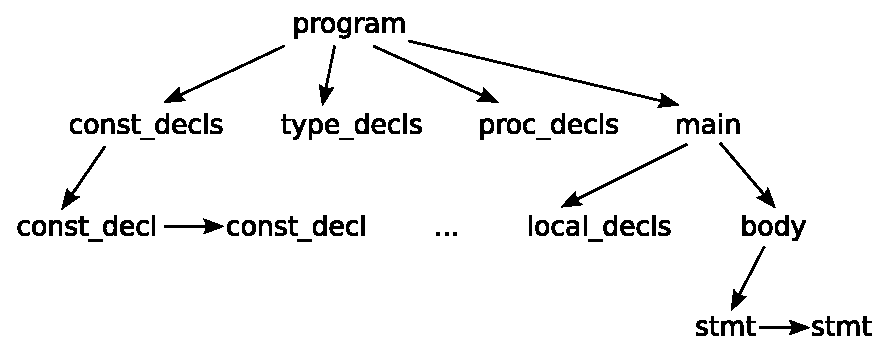
\psfig{file=figs/top_down_parse.eps,width=20em}
\end{center}

One can (easily) write a predictive parser by hand, or generate one
from an LL({\em k}) grammar:
\begin{itemize}
\item {\em \underline{L}eft-to-right parse};
\item {\em \underline{L}eftmost-derivation}; and
\item {\em \underline{k} symbol lookahead}.
\end{itemize}

Algorithm: look at beginning of input (up to {\em k} characters) and
unambiguously expand leftmost non-terminal.

\vfil
\end{slide*}

\begin{slide*}
2) \underline{Bottom-up} parsers.

\vspace{0.1in}

Algorithm: look for a sequence matching RHS and reduce to LHS.
Postpone any decision until entire RHS is seen, plus {\em k} tokens
lookahead.

Can write a bottom-up parser by hand (tricky), or generate one
from an LR({\em k}) grammar (easy):
\begin{itemize}
\item {\em \underline{L}eft-to-right parse};
\item {\em \underline{R}ightmost-derivation}; and
\item {\em \underline{k} symbol lookahead}.
\end{itemize}

\vspace{0.1in}

\begin{center}
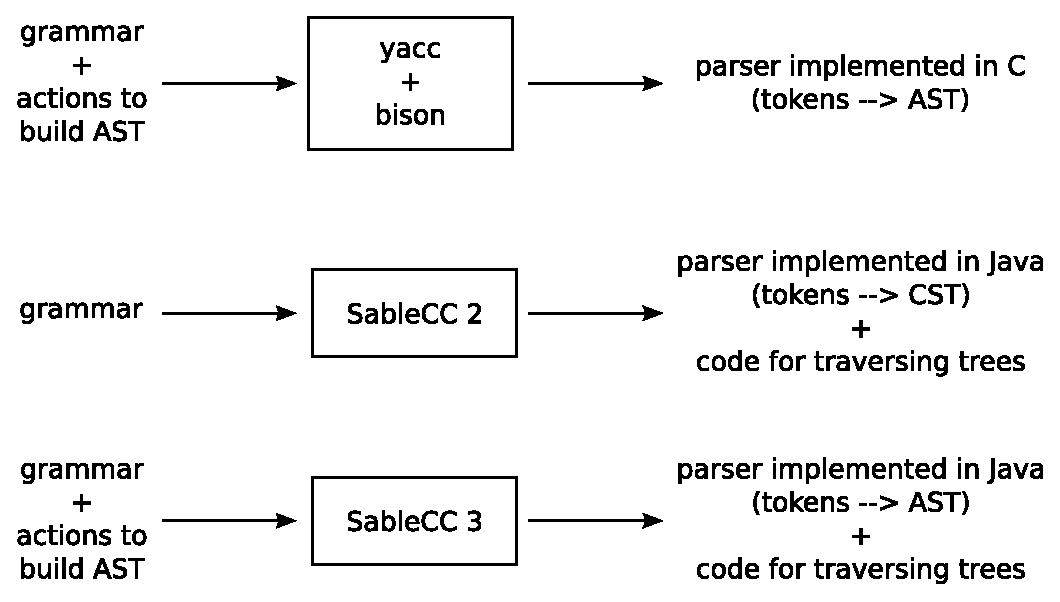
\psfig{file=figs/grammar_to_parser.eps,width=20em}
\end{center}

\vfil
\end{slide*}

\begin{slide*}
The {\em shift-reduce} bottom-up parsing technique.

1) Extend the grammar with an end-of-file \$, introduce fresh start symbol $S'$:

\begin{tabular}{lll}
$S'$ \RA $S$\$ & & \\
$S$ \RA{} $S$ ; $S$ & $E$ \RA{} id & $L$ \RA{} $E$ \\
$S$ \RA{} id := $E$ & $E$ \RA{} num & $L$ \RA{} $L$ , $E$\\
$S$ \RA{} print ( $L$ ) & $E$ \RA{} $E$ + $E$ & \\
 & $E$ \RA{} ( $S$ , $E$ ) &
\end{tabular}

2) Choose between the following actions:
\begin{itemize}
\item shift:\\ move first input token to top of stack
\item reduce:\\ replace $\alpha$ on top of stack by $X$\\ for some rule $X$\RA{} $\alpha$
\item accept:\\ when $S'$ is on the stack
\end{itemize}

\vfil
\end{slide*}

\begin{slide*}
\begin{minipage}[t]{1.5cm}
\renewcommand{\arraystretch}{0.7}
\begin{small}
\begin{tabular}[t]{l}
~\\
id\\
id :=\\
id := num\\
id := $E$\\
$S$\\
$S$;\\
$S$; id\\
$S$; id :=\\
$S$; id := id\\
$S$; id := $E$\\
$S$; id := $E$ +\\
$S$; id := $E$ + (\\
$S$; id := $E$ + ( id\\
$S$; id := $E$ + ( id :=\\
$S$; id := $E$ + ( id := num\\
$S$; id := $E$ + ( id := $E$\\
$S$; id := $E$ + ( id := $E$ +\\
$S$; id := $E$ + ( id := $E$ + num\\
$S$; id := $E$ + ( id := $E$ + $E$\\
$S$; id := $E$ + ( id := $E$\\
$S$; id := $E$ + ( $S$\\
$S$; id := $E$ + ( $S$,\\
$S$; id := $E$ + ( $S$, id\\
$S$; id := $E$ + ( $S$, $E$\\
$S$; id := $E$ + ( $S$, $E$ )\\
$S$; id := $E$ + $E$\\
$S$; id := $E$\\
$S$; $S$\\
$S$\\
$S$\$\\
$S'$
\end{tabular}
\end{small}
\end{minipage}
\begin{minipage}[t]{4cm}
\renewcommand{\arraystretch}{0.71}
\begin{small}
\begin{tabular}[t]{r}
{\tt a:=7; b:=c+(d:=5+6,d)\$}\\
{\tt :=7; b:=c+(d:=5+6,d)\$}\\
{\tt 7; b:=c+(d:=5+6,d)\$}\\
{\tt ; b:=c+(d:=5+6,d)\$}\\
{\tt ; b:=c+(d:=5+6,d)\$}\\
{\tt ; b:=c+(d:=5+6,d)\$}\\
{\tt b:=c+(d:=5+6,d)\$}\\
{\tt :=c+(d:=5+6,d)\$}\\
{\tt c+(d:=5+6,d)\$}\\
{\tt +(d:=5+6,d)\$}\\
{\tt +(d:=5+6,d)\$}\\
{\tt (d:=5+6,d)\$}\\
{\tt d:=5+6,d)\$}\\
{\tt :=5+6,d)\$}\\
{\tt 5+6,d)\$}\\
{\tt +6,d)\$}\\
{\tt +6,d)\$}\\
{\tt 6,d)\$}\\
{\tt ,d)\$}\\
{\tt ,d)\$}\\
{\tt ,d)\$}\\
{\tt ,d)\$}\\
{\tt d)\$}\\
{\tt )\$}\\
{\tt )\$}\\
{\tt \$}\\
{\tt \$}\\
{\tt \$}\\
{\tt \$}\\
{\tt \$}\\
\\
\end{tabular}
\end{small}
\end{minipage}
\begin{minipage}[t]{1cm}
\renewcommand{\arraystretch}{0.71}
\begin{small}
\begin{tabular}[t]{l}
shift\\
shift\\
shift\\
$E$\RA{}num\\
$S$\RA{}id:=$E$\\
shift\\
shift\\
shift\\
shift\\
$E$\RA{}id\\
shift\\
shift\\
shift\\
shift\\
shift\\
$E$\RA{}num\\
shift\\
shift\\
$E$\RA{}num\\
$E$\RA{}$E$+$E$\\
$S$\RA{}id:=$E$\\
shift\\
shift\\
$E$\RA{}id\\
shift\\
$E$\RA{}($S$;$E$)\\
$E$\RA{}$E$+$E$\\
$S$\RA{}id:=$E$\\
$S$\RA{}$S$;$S$\\
shift\\
$S'$\RA{}$S$\$\\
accept
\end{tabular}
\end{small}
\end{minipage}
\vfil
\end{slide*}

\begin{slide*}
\begin{tabular}{ll}
$_0$ $S'$ \RA $S$\$ & $_5$ $E$ \RA{} num\\
$_1$ $S$ \RA{} $S$ ; $S$ & $_6$ $E$ \RA{} $E$ + $E$\\
$_2$ $S$ \RA{} id := $E$ & $_7$ $E$ \RA{} ( $S$ , $E$ )\\
$_3$ $S$ \RA{} print ( $L$ ) & $_8$ $L$ \RA{} $E$ \\
$_4$ $E$ \RA{} id & $_9$ $L$ \RA{} $L$ , $E$
\end{tabular}

Use a DFA to choose the action;
the stack only contains DFA states now.

Start with the initial state (s1) on the stack.

Lookup (stack top, next input symbol):
\begin{itemize}
\item shift($n$): skip next input symbol and push state $n$
\item reduce($k$): rule $k$ is $X$\RA{}$\alpha$; pop $|\alpha|$ times; 
                   lookup (stack top, $X$) in table
\item goto($n$): push state $n$
\item accept: report success
\item error: report failure
\end{itemize}

\vfil
\end{slide*}

\begin{slide*}
\begin{scriptsize}
\newcommand{\squeeze}{\hspace{0.4em}}
\begin{tabular}{c@{\squeeze}|c@{\squeeze}c@{\squeeze}c@{\squeeze}c@{\squeeze}c@{\squeeze}c@{\squeeze}c@{\squeeze}c@{\squeeze}c@{\squeeze}c@{\squeeze}|c@{\squeeze}c@{\squeeze}c@{\squeeze}}
DFA & \multicolumn{10}{c|}{terminals} &
\multicolumn{3}{c}{non-terminals}\\\cline{2-14}

state & id & num & print &  ; &  , &  + &  := &  ( &  ) & \$ & $S$ & $E$ & $L$\\\hline
 1 & s4 &     &  s7   &    &    &    &     &    &    &    &  g2 &     &    \\
 2 &    &     &       & s3 &    &    &     &    &    &  a &     &     &    \\
 3 & s4 &     &  s7   &    &    &    &     &    &    &    &  g5 &     &    \\
 4 &    &     &       &    &    &    &  s6 &    &    &    &     &     &    \\
 5 &    &     &       & r1 & r1 &    &     &    &    & r1 &     &     &    \\\hline
 6 & s20& s10 &       &    &    &    &     & s8 &    &    &     & g11 &    \\
 7 &    &     &       &    &    &    &     & s9 &    &    &     &     &    \\
 8 & s4 &     &  s7   &    &    &    &     &    &    &    & g12 &     &    \\
 9 &    &     &       &    &    &    &     &    &    &    &     & g15 & g14\\
 10&    &     &       & r5 & r5 & r5 &     &    & r5 & r5 &     &     &    \\\hline
 11&    &     &       & r2 & r2 & s16&     &    &    & r2 &     &     &    \\
 12&    &     &       & s3 & s18&    &     &    &    &    &     &     &    \\
 13&    &     &       & r3 & r3 &    &     &    &    & r3 &     &     &    \\
 14&    &     &       &    & s19&    &     &    & s13&    &     &     &    \\
 15&    &     &       &    & r8 &    &     &    & r8 &    &     &     &    \\\hline
 16&s20 & s10 &       &    &    &    &     & s8 &    &    &     & g17 &    \\
 17&    &     &       & r6 & r6 & s16&     &    & r6 & r6 &     &     &    \\
 18&s20 & s10 &       &    &    &    &     & s8 &    &    &     & g21 &    \\
 19&s20 & s10 &       &    &    &    &     & s8 &    &    &     & g23 &    \\
 20&    &     &       & r4 & r4 & r4 &     &    & r4 & r4 &     &     &    \\\hline
 21&    &     &       &    &    &    &     &    & s22&    &     &     &    \\
 22&    &     &       & r7 & r7 & r7 &     &    & r7 & r7 &     &     &    \\
 23&    &     &       &    & r9 & s16&     &    & r9 &    &     &     &    
\end{tabular}
\end{scriptsize}

\vspace{-0.05in}
\begin{small}
Error transitions omitted.
\end{small}
\vfil
\end{slide*}

\begin{slide*}
\begin{center}
\begin{tabular}{lp{1cm}r}
$s_1$ && a := 7\$\\
shift(4)\\
$s_1 ~s_4$ && := 7\$\\
shift(6)\\
$s_1 ~s_4 ~s_6$ && 7\$\\
shift(10)\\
$s_1 ~s_4 ~s_6 ~s_{10}$ && \$\\
reduce(5): $E$ \RA{} num\\
~~~$s_1 ~s_4 ~s_6 \xout{~s_{10}}$ && \$\\
~~~lookup($s_6$,$E$) = goto(11)\\
$s_1 ~s_4 ~s_6 ~s_{11}$ && \$\\
reduce(2): $S$ \RA{} id := $E$\\
~~~$s_1 \xout{~s_4} \xout{~s_6} \xout{~s_{11}}$ && \$\\
~~~lookup($s_1$,$S$) = goto(2)\\
$s_1 ~s_2$ && \$\\
accept
\end{tabular} 
\end{center}
\end{slide*}


\begin{slide*}
LR(1) is an algorithm that attempts to construct a parsing table:
\begin{itemize}
\item {\em \underline{L}eft-to-right parse};
\item {\em \underline{R}ightmost-derivation}; and
\item {\em \underline{1} symbol lookahead}.
\end{itemize}
If no conflicts (shift/reduce, reduce/reduce) arise, then we are happy;
otherwise, fix grammar.

\vspace{0.1in}

An LR(1) item (A \RA{} $\alpha$ . $\beta\gamma$, x) consists of
\begin{enumerate}
\item A grammar production, A \RA{} $\alpha\beta\gamma$
\item The RHS position, represented by '.'
\item A lookahead symbol, x
\end{enumerate}

An LR(1) state is a set of LR(1) items.

\vspace{0.1in}

The sequence $\alpha$ is on top of the stack, and the head of the
input is derivable from $\beta\gamma$x.  There are two cases for $\beta$,
terminal or non-terminal.
\vfil
\end{slide*}

\begin{slide*}
We first compute a set of LR(1) states from our grammar, and then use
them to build a parse table.  There are four kinds of entry to make:
\begin{enumerate}
\item goto: when $\beta$ is non-terminal
\item shift: when $\beta$ is terminal
\item reduce: when $\beta$ is empty (the next state is the number of
  the production used)
\item accept: when we have A \RA{} B . \$
\end{enumerate}

\vspace{0.1in}

Follow construction on the tiny grammar:

\begin{tabular}{l@{~~~~~~~}l}
$_0$ $S$ \RA{} $E$\$ & $_2$ $E$ \RA{} $T$\\
$_1$ $E$ \RA{} $T$ + $E$ & $_3$ $T$ \RA{} x
\end{tabular}

\vspace{0.1in}

% Don't worry about constructing the LR states, but do understand how
% to build the parse table from the state diagram.  (It's not hard.)
% 
% \vspace{0.1in}

\vfil
\end{slide*}



\begin{slide*}
\newcommand{\lritem}[2]{
\fbox{
\begin{minipage}[b]{1.9cm}#1\end{minipage}
\begin{minipage}[b]{5mm}\begin{tabular}{r}#2\end{tabular}\end{minipage}
}
}
Constructing the LR(1) NFA:
\begin{itemize} 
  \item start with state~ \lritem{$S$\RA{}~.~$E$\$}{?}
  \item state \lritem{$A$\RA{}$\alpha$~.~$B~\beta$}{l} has:\\[1.5ex]
\begin{itemize} 
  \item $\epsilon$-successor \lritem{$B$\RA{}~.~$\gamma$}{x}, if:\\
  \begin{itemize} 
	  \item exists rule \mbox{$B$ \RA{} $\gamma$}, and
	  \item x~$\in$~lookahead($\beta$)
  \end{itemize}
  \item $B$-successor \lritem{$A$\RA{}$\alpha~B~$.$~\beta$}{l}\\
\end{itemize}
  \item state \lritem{$A$\RA{}$\alpha$~.~x$~\beta$}{l} has:\\[1.5ex]
  	x-successor \lritem{$A$\RA{}$\alpha~$x~.$~\beta$}{l}\\
\end{itemize}
\vfil
Constructing the LR(1) DFA:\\
Standard power-set construction, ``inlining'' $\epsilon$-transitions.
\vfil
\end{slide*}

\begin{slide*}
\newcommand{\lritem}[2]{
\hspace*{-0.36cm}
\begin{minipage}[b]{1.9cm}#1\end{minipage}
\begin{minipage}[b]{1cm}\begin{tabular}{r}#2\end{tabular}\end{minipage}
}
\setlength{\unitlength}{0.00083300in}%
%
\begingroup\makeatletter\ifx\SetFigFont\undefined%
\gdef\SetFigFont#1#2#3#4#5{%
  \reset@font\fontsize{#1}{#2pt}%
  \fontfamily{#3}\fontseries{#4}\fontshape{#5}%
  \selectfont}%
\fi\endgroup%
\begin{picture}(3225,2883)(1951,-3523)
\thicklines
\put(2101,-1786){\framebox(1200,1125){}}
\put(2176,-886){\makebox(0,0)[lb]{\smash{\SetFigFont{12}{14.4}{\familydefault}{\mddefault}{\updefault}\lritem{$S$\RA{}.$E$\$}{?}}}}
\put(2176,-1096){\makebox(0,0)[lb]{\smash{\SetFigFont{12}{14.4}{\familydefault}{\mddefault}{\updefault}\lritem{$E$\RA{}.$T$+$E$}{\$}}}}
\put(2176,-1306){\makebox(0,0)[lb]{\smash{\SetFigFont{12}{14.4}{\familydefault}{\mddefault}{\updefault}\lritem{$E$\RA{}.$T$}{\$}}}}
\put(2176,-1516){\makebox(0,0)[lb]{\smash{\SetFigFont{12}{14.4}{\familydefault}{\mddefault}{\updefault}\lritem{$T$\RA{}.x}{\hspace*{-0.08cm}+}}}}
\put(2176,-1726){\makebox(0,0)[lb]{\smash{\SetFigFont{12}{14.4}{\familydefault}{\mddefault}{\updefault}\lritem{$T$\RA{}.x}{\$}}}}
\put(3901,-1786){\framebox(1200,525){}}
\put(3976,-1486){\makebox(0,0)[lb]{\smash{\SetFigFont{12}{14.4}{\familydefault}{\mddefault}{\updefault}\lritem{$E$\RA{}$T$.+$E$}{\$}}}}
\put(3976,-1696){\makebox(0,0)[lb]{\smash{\SetFigFont{12}{14.4}{\familydefault}{\mddefault}{\updefault}\lritem{$E$\RA{}$T$.}{\$}}}}
\put(3901,-961){\framebox(1200,300){}}
\put(3976,-886){\makebox(0,0)[lb]{\smash{\SetFigFont{12}{14.4}{\familydefault}{\mddefault}{\updefault}\lritem{$S$\RA{}$E$.\$}{?}}}}
\put(3901,-3511){\framebox(1200,1125){}}
\put(3976,-2611){\makebox(0,0)[lb]{\smash{\SetFigFont{12}{14.4}{\familydefault}{\mddefault}{\updefault}\lritem{$E$\RA{}$T$+.$E$}{\$}}}}
\put(3976,-2821){\makebox(0,0)[lb]{\smash{\SetFigFont{12}{14.4}{\familydefault}{\mddefault}{\updefault}\lritem{$E$\RA{}.$T$+$E$}{\$}}}}
\put(3976,-3031){\makebox(0,0)[lb]{\smash{\SetFigFont{12}{14.4}{\familydefault}{\mddefault}{\updefault}\lritem{$E$\RA{}.$T$}{\$}}}}
\put(3976,-3241){\makebox(0,0)[lb]{\smash{\SetFigFont{12}{14.4}{\familydefault}{\mddefault}{\updefault}\lritem{$T$\RA{}.x}{\$}}}}
\put(3976,-3451){\makebox(0,0)[lb]{\smash{\SetFigFont{12}{14.4}{\familydefault}{\mddefault}{\updefault}\lritem{$T$\RA{}.x}{\hspace*{-0.08cm}+}}}}
\put(2101,-2911){\framebox(1200,525){}}
\put(2176,-2611){\makebox(0,0)[lb]{\smash{\SetFigFont{12}{14.4}{\familydefault}{\mddefault}{\updefault}\lritem{$T$\RA{}x.}{\hspace*{-0.08cm}+}}}}
\put(2176,-2821){\makebox(0,0)[lb]{\smash{\SetFigFont{12}{14.4}{\familydefault}{\mddefault}{\updefault}\lritem{$T$\RA{}x.}{\$}}}}
\put(2101,-3511){\framebox(1200,300){}}
\put(2176,-3436){\makebox(0,0)[lb]{\smash{\SetFigFont{12}{14.4}{\familydefault}{\mddefault}{\updefault}\lritem{$E$\RA{}$T$+$E$.}{\$}}}}
\put(3301,-811){\vector( 1, 0){600}}
\put(3301,-1486){\vector( 1, 0){600}}
\put(4201,-1786){\vector( 0,-1){600}}
\put(4801,-2386){\vector( 0, 1){600}}
\put(2701,-1786){\vector( 0,-1){600}}
\put(3901,-2611){\vector(-1, 0){600}}
\put(3901,-3361){\vector(-1, 0){600}}
\put(1951,-886){\makebox(0,0)[lb]{\smash{\SetFigFont{12}{14.4}{\familydefault}{\mddefault}{\updefault}1}}}
\put(5176,-886){\makebox(0,0)[lb]{\smash{\SetFigFont{12}{14.4}{\familydefault}{\mddefault}{\updefault}2}}}
\put(5176,-1486){\makebox(0,0)[lb]{\smash{\SetFigFont{12}{14.4}{\familydefault}{\mddefault}{\updefault}3}}}
\put(5176,-2611){\makebox(0,0)[lb]{\smash{\SetFigFont{12}{14.4}{\familydefault}{\mddefault}{\updefault}4}}}
\put(1951,-2611){\makebox(0,0)[lb]{\smash{\SetFigFont{12}{14.4}{\familydefault}{\mddefault}{\updefault}5}}}
\put(1951,-3436){\makebox(0,0)[lb]{\smash{\SetFigFont{12}{14.4}{\familydefault}{\mddefault}{\updefault}6}}}
\put(3526,-736){\makebox(0,0)[lb]{\smash{\SetFigFont{12}{14.4}{\familydefault}{\mddefault}{\updefault}$E$}}}
\put(3526,-1411){\makebox(0,0)[lb]{\smash{\SetFigFont{12}{14.4}{\familydefault}{\mddefault}{\updefault}$T$}}}
\put(2551,-2161){\makebox(0,0)[lb]{\smash{\SetFigFont{12}{14.4}{\familydefault}{\mddefault}{\updefault}x}}}
\put(4051,-2161){\makebox(0,0)[lb]{\smash{\SetFigFont{12}{14.4}{\familydefault}{\mddefault}{\updefault}+}}}
\put(4876,-2161){\makebox(0,0)[lb]{\smash{\SetFigFont{12}{14.4}{\familydefault}{\mddefault}{\updefault}$T$}}}
\put(3526,-2536){\makebox(0,0)[lb]{\smash{\SetFigFont{12}{14.4}{\familydefault}{\mddefault}{\updefault}x}}}
\put(3526,-3286){\makebox(0,0)[lb]{\smash{\SetFigFont{12}{14.4}{\familydefault}{\mddefault}{\updefault}$E$}}}
\end{picture}
\vfil
\begin{small}
\begin{tabular}{l|ccc|cc}
  & x   & +  & \$  &  $E$  &  $T$  \\\hline
1 & s5  &    &     &  g2   &  g3   \\
2 &     &    & a   &       &       \\
3 &     & s4 & r2  &       &       \\
4 & s5  &    &     &  g6   &  g3   \\
5 &     & r3 & r3  &       &       \\
6 &     &    & r1  &       &       
\end{tabular}
\end{small}
\vfil
\end{slide*}

\begin{slide*}
\newcommand{\lritem}[2]{
\hspace*{-0.36cm}
\begin{minipage}[b]{1.9cm}#1\end{minipage}
\begin{minipage}[b]{1cm}\begin{tabular}{r}#2\end{tabular}\end{minipage}
}
\setlength{\unitlength}{0.00083300in}%
%
\begingroup\makeatletter\ifx\SetFigFont\undefined%
\gdef\SetFigFont#1#2#3#4#5{%
  \reset@font\fontsize{#1}{#2pt}%
  \fontfamily{#3}\fontseries{#4}\fontshape{#5}%
  \selectfont}%
\fi\endgroup%
Conflicts\\[1.5ex]
\begin{picture}(3225,700)(1951,-1200)
\thicklines
\put(2101,-1186){\framebox(1230,525){}}
\put(2176,-886){\makebox(0,0)[lb]{\smash{\SetFigFont{12}{14.4}{\familydefault}{\mddefault}{\updefault}\lritem{$A$\RA{}.$B$}{x}}}}
\put(2176,-1096){\makebox(0,0)[lb]{\smash{\SetFigFont{12}{14.4}{\familydefault}{\mddefault}{\updefault}\lritem{$A$\RA{}$C$.}{y}}}}
\put(3500,-1000){no conflict (lookahead decides)}
\end{picture}
\begin{picture}(3225,700)(1951,-1200)
\thicklines
\put(2101,-1186){\framebox(1230,525){}}
\put(2176,-886){\makebox(0,0)[lb]{\smash{\SetFigFont{12}{14.4}{\familydefault}{\mddefault}{\updefault}\lritem{$A$\RA{}.$B$}{x}}}}
\put(2176,-1096){\makebox(0,0)[lb]{\smash{\SetFigFont{12}{14.4}{\familydefault}{\mddefault}{\updefault}\lritem{$A$\RA{}$C$.}{x}}}}
\put(3500,-1000){shift/reduce conflict}
\end{picture}
\begin{picture}(3225,700)(1951,-1200)
\thicklines
\put(2101,-1186){\framebox(1230,525){}}
\put(2176,-886){\makebox(0,0)[lb]{\smash{\SetFigFont{12}{14.4}{\familydefault}{\mddefault}{\updefault}\lritem{$A$\RA{}.x}{y}}}}
\put(2176,-1096){\makebox(0,0)[lb]{\smash{\SetFigFont{12}{14.4}{\familydefault}{\mddefault}{\updefault}\lritem{$A$\RA{}$C$.}{x}}}}
\put(3500,-1000){shift/reduce conflict}
\end{picture}
\begin{picture}(3225,700)(1951,-1200)
\thicklines
\put(2101,-1186){\framebox(1230,525){}}
\put(2176,-886){\makebox(0,0)[lb]{\smash{\SetFigFont{12}{14.4}{\familydefault}{\mddefault}{\updefault}\lritem{$A$\RA{}$B$.}{x}}}}
\put(2176,-1096){\makebox(0,0)[lb]{\smash{\SetFigFont{12}{14.4}{\familydefault}{\mddefault}{\updefault}\lritem{$A$\RA{}$C$.}{x}}}}
\put(3500,-1000){reduce/reduce conflict}
\end{picture}\\[5mm]
\begin{picture}(3225,700)(1951,-1200)
\thicklines
\put(2101,-1186){\framebox(1230,525){}}
\put(2176,-886){\makebox(0,0)[lb]{\smash{\SetFigFont{12}{14.4}{\familydefault}{\mddefault}{\updefault}\lritem{$A$\RA{}.$B$}{x}}}}
\put(2176,-1096){\makebox(0,0)[lb]{\smash{\SetFigFont{12}{14.4}{\familydefault}{\mddefault}{\updefault}\lritem{$A$\RA{}.$C$}{x}}}}
\put(3331,-811){\vector( 1, 0){600} $s_i$}
\put(3331,-1061){\vector( 1, 0){600} $s_j$}
\put(3381,-750){$B$}
\put(3381,-1000){$C$}
\end{picture}\\[1.5ex]
\hspace*{5mm}shift/shift conflict?\\
\hspace*{5mm}$\Rightarrow$ by construction of the \underbar{D}FA \\
\hspace*{1cm}we have $s_i=s_j$ 
\vfil 
\end{slide*}

\begin{slide*}
LR(1) tables may become very large.

Parser generators use LALR(1), which merges states that are identical
except for lookaheads.

\begin{center}
~\\
\setlength{\unitlength}{0.00065in}%
%
\begingroup\makeatletter\ifx\SetFigFont\undefined%
\gdef\SetFigFont#1#2#3#4#5{%
  \reset@font\fontsize{#1}{#2pt}%
  \fontfamily{#3}\fontseries{#4}\fontshape{#5}%
  \selectfont}%
\fi\endgroup%
\begin{picture}(4449,4224)(1264,-5473)
\thicklines
\put(2401,-4261){\framebox(1500,900){}}
\put(2551,-4111){\framebox(600,600){}}
\put(2101,-4711){\framebox(2100,1875){}}
\put(1726,-5011){\framebox(3000,2700){}}
\put(1501,-5236){\framebox(3750,3450){}}
\put(1276,-5461){\framebox(4425,4200){}}
\put(2251,-4561){\framebox(1050,2625){}}
\put(2176,-4636){\framebox(1200,3300){}}
\put(2626,-3886){\makebox(0,0)[lb]{\smash{\SetFigFont{8}{14.4}{\familydefault}{\mddefault}{\updefault}LL(0)}}}
\put(3601,-3211){\makebox(0,0)[lb]{\smash{\SetFigFont{8}{14.4}{\familydefault}{\mddefault}{\updefault}SLR}}}
\put(3901,-2686){\makebox(0,0)[lb]{\smash{\SetFigFont{8}{14.4}{\familydefault}{\mddefault}{\updefault}LALR(1)}}}
\put(4351,-2161){\makebox(0,0)[lb]{\smash{\SetFigFont{8}{14.4}{\familydefault}{\mddefault}{\updefault}LR(1)}}}
\put(4651,-1636){\makebox(0,0)[lb]{\smash{\SetFigFont{8}{14.4}{\familydefault}{\mddefault}{\updefault}LR(k)}}}
\put(2551,-1636){\makebox(0,0)[lb]{\smash{\SetFigFont{8}{14.4}{\familydefault}{\mddefault}{\updefault}LL(k)}}}
\put(2551,-2161){\makebox(0,0)[lb]{\smash{\SetFigFont{8}{14.4}{\familydefault}{\mddefault}{\updefault}LL(1)}}}
\put(3451,-3886){\makebox(0,0)[lb]{\smash{\SetFigFont{8}{14.4}{\familydefault}{\mddefault}{\updefault}LR(0)}}}
\end{picture}
\end{center}
\vfil
\end{slide*}

\begin{slide*}
{\tt bison} ({\tt yacc}) is a parser generator:
\begin{itemize}
\item it inputs a grammar;
\item it computes an LALR(1) parser table;
\item it reports conflicts;
\item it resolves conflicts using defaults (!); and
\item it creates a C program.
\end{itemize}
\vspace*{2em}

Nobody writes (simple) parsers by hand anymore.
\vfil
\end{slide*}

\begin{slide*}
The grammar:

\begin{tabular}{l@{~~~~}l@{~~~~}l}
$_1$ $E$ \RA{} id & $_4$ $E$ \RA{} $E$ $/$ $E$ & $_7$ $E$ \RA{} ( $E$ )\\
$_2$ $E$ \RA{} num & $_5$ $E$ \RA{} $E$ + $E$ & \\
$_3$ $E$ \RA{} $E$ $*$ $E$ & $_6$ $E$ \RA{} $E$ $-$ $E$ & \\
\end{tabular}

is expressed in {\tt bison} as:

\begin{scriptsize}
\begin{verbatim}
%{
/* C declarations */
%}

/* Bison declarations; tokens come from lexer (scanner) */
%token tIDENTIFIER tINTCONST

%start exp

/* Grammar rules after the first %% */
%%
exp : tIDENTIFIER
    | tINTCONST
    | exp '*' exp
    | exp '/' exp
    | exp '+' exp
    | exp '-' exp
    | '(' exp ')'
;
%%
/* User C code after the second %% */
\end{verbatim}
\end{scriptsize}
Input this code into exp.y to follow the example.
\vfil
\end{slide*}

\begin{slide*}
The grammar is ambiguous:

\begin{scriptsize}
\begin{verbatim}
$ bison --verbose exp.y # --verbose produces exp.output
exp.y contains 16 shift/reduce conflicts.

$ cat exp.output
State 11 contains 4 shift/reduce conflicts.
State 12 contains 4 shift/reduce conflicts.
State 13 contains 4 shift/reduce conflicts.
State 14 contains 4 shift/reduce conflicts.

[...]

state 11
 
    exp  ->  exp . '*' exp   (rule 3)
    exp  ->  exp '*' exp .   (rule 3) <-- problem is here
    exp  ->  exp . '/' exp   (rule 4)
    exp  ->  exp . '+' exp   (rule 5)
    exp  ->  exp . '-' exp   (rule 6)
 
    '*'         shift, and go to state 6
    '/'         shift, and go to state 7
    '+'         shift, and go to state 8
    '-'         shift, and go to state 9
 
    '*'         [reduce using rule 3 (exp)]
    '/'         [reduce using rule 3 (exp)]
    '+'         [reduce using rule 3 (exp)]
    '-'         [reduce using rule 3 (exp)]
    $default    reduce using rule 3 (exp)
\end{verbatim}
\end{scriptsize}
\vfil
\end{slide*}

\begin{slide*}
Rewrite the grammar to force reductions:

\begin{tabular}{l@{~~~~~~}l@{~~~~~~}l}
$E$ \RA{} $E$ + $T$ & $T$ \RA{} $T$ $*$ $F$ & $F$ \RA{} id\\
$E$ \RA{} $E$ - $T$ & $T$ \RA{} $T$ $/$ $F$ & $F$ \RA{} num\\
$E$ \RA{} $T$ & $T$ \RA{} $F$ & $F$ \RA{} ( $E$ ) 
\end{tabular}

\begin{scriptsize}
\begin{verbatim}

%token tIDENTIFIER tINTCONST

%start exp

%% 
exp : exp '+' term
    | exp '-' term
    | term
;

term : term '*' factor
     | term '/' factor
     | factor
;

factor : tIDENTIFIER
       | tINTCONST
       | '(' exp ')'
;
%%
\end{verbatim}
\end{scriptsize}
\vfil
\end{slide*}

\begin{slide*}
Or use precedence directives:

\begin{scriptsize}
\begin{verbatim}
%token tIDENTIFIER tINTCONST

%start exp

%left '+' '-'    /* left-associative, lower precedence */
%left '*' '/'    /* left-associative, higher precedence */

%% 
exp : tIDENTIFIER
    | tINTCONST
    | exp '*' exp
    | exp '/' exp
    | exp '+' exp
    | exp '-' exp
    | '(' exp ')'
;
%%
\end{verbatim}
\end{scriptsize}

which resolve shift/reduce conflicts:

\begin{scriptsize}
\begin{verbatim}
Conflict in state 11 between rule 5 and token '+' 
         resolved as reduce. <-- Reduce exp + exp . +
Conflict in state 11 between rule 5 and token '-' 
         resolved as reduce. <-- Reduce exp + exp . -
Conflict in state 11 between rule 5 and token '*' 
         resolved as shift.  <-- Shift exp + exp . *
Conflict in state 11 between rule 5 and token '/' 
         resolved as shift.  <-- Shift exp + exp . /
\end{verbatim}
\end{scriptsize}
Note that this is not the same state 11 as before.
\vfil
\end{slide*}

\begin{slide*}
The precedence directives are:
\begin{itemize}
\item {\tt \%left} {\em (left-associative)}
\item {\tt \%right} {\em (right-associative)}
\item {\tt \%nonassoc} {\em (non-associative)}
\end{itemize}
When constructing a parse table, an action is chosen based on the
precedence of the last symbol on the right-hand side of the rule.

\vspace{0.1in}

Precedences are ordered from lowest to highest on a linewise basis.

\vspace{0.1in}

If precedences are equal, then:
\begin{itemize}
\item {\tt \%left~} favors reducing
\item {\tt \%right~} favors shifting
\item {\tt \%nonassoc~} yields an error
\end{itemize}
This usually ends up working.
\vfil
\end{slide*}

\begin{slide*}
\begin{scriptsize}
\begin{verbatim}
state 0
    tIDENTIFIER shift, and go to state 1
    tINTCONST   shift, and go to state 2
    '('         shift, and go to state 3
    exp         go to state 4

state 1
    exp  ->  tIDENTIFIER .   (rule 1)
    $default    reduce using rule 1 (exp)

state 2
    exp  ->  tINTCONST .   (rule 2)
    $default    reduce using rule 2 (exp)

.
.
.

state 14
    exp  ->  exp . '*' exp   (rule 3)
    exp  ->  exp . '/' exp   (rule 4)
    exp  ->  exp '/' exp .   (rule 4)
    exp  ->  exp . '+' exp   (rule 5)
    exp  ->  exp . '-' exp   (rule 6)
    $default    reduce using rule 4 (exp)
 
state 15
    $           go to state 16
 
state 16
    $default    accept
\end{verbatim}
\end{scriptsize}
\vfil
\end{slide*}

\begin{slide*}
\begin{scriptsize}
\begin{verbatim}
$ cat exp.y
%{
#include <stdio.h>   /* for printf */

extern char *yytext; /* string from scanner */
void yyerror() {
  printf ("syntax error before %s\n", yytext); 
}
%}
 
%union {
   int intconst;
   char *stringconst;
}
 
%token <intconst> tINTCONST
%token <stringconst> tIDENTIFIER 
 
%start exp
 
%left '+' '-'
%left '*' '/'
 
%% 
exp : tIDENTIFIER { printf ("load %s\n", $1); }
    | tINTCONST   { printf ("push %i\n", $1); }
    | exp '*' exp { printf ("mult\n"); }
    | exp '/' exp { printf ("div\n"); }
    | exp '+' exp { printf ("plus\n"); }
    | exp '-' exp { printf ("minus\n"); }
    | '(' exp ')' {}
;
%%
\end{verbatim}
\end{scriptsize}
\vfil
\end{slide*}

\begin{slide*}
\begin{scriptsize}
\begin{verbatim}
$ cat exp.l
%{
#include "y.tab.h"  /* for exp.y types */
#include <string.h> /* for strlen */
#include <stdlib.h> /* for malloc and atoi */
%}
 
%%
[ \t\n]+  /* ignore */;
 
"*"       return '*';
"/"       return '/';
"+"       return '+';
"-"       return '-';
"("       return '(';
")"       return ')';
 
0|([1-9][0-9]*) { 
  yylval.intconst = atoi (yytext);
  return tINTCONST; 
}

[a-zA-Z_][a-zA-Z0-9_]* { 
  yylval.stringconst = 
    (char *) malloc (strlen (yytext) + 1);
  sprintf (yylval.stringconst, "%s", yytext); 
  return tIDENTIFIER;
}

.         /* ignore */
%%
\end{verbatim}
\end{scriptsize}
\vfil
\end{slide*}

\begin{slide*}
\begin{scriptsize}
\begin{verbatim}
$ cat main.c
void yyparse();

int main (void)
{ 
  yyparse ();
}
\end{verbatim}
\end{scriptsize}

\vspace{1em}

Using {\tt flex}/{\tt bison} to create a parser is simple:
\begin{scriptsize}
\begin{verbatim}
$ flex exp.l
$ bison --yacc --defines exp.y # note compatability options
$ gcc lex.yy.c y.tab.c y.tab.h main.c -o exp -lfl
\end{verbatim}
\end{scriptsize}

\vspace{1em}

When input {\tt a*(b-17) + 5/c}:

\begin{scriptsize}
\begin{verbatim}
$ echo "a*(b-17) + 5/c" | ./exp
\end{verbatim}
\end{scriptsize}

our {\tt exp} parser outputs the correct order of operations:

\begin{scriptsize}
\begin{verbatim}
load a
load b
push 17
minus
mult
push 5
load c
div
plus
\end{verbatim}
\end{scriptsize}

You should confirm this for yourself!
\vfil
\end{slide*}

\begin{slide*}
If the input contains syntax errors, then the {\tt bison}-generated
parser calls {\tt yyerror} and stops.

We may ask it to recover from the error:
 
\begin{scriptsize}
\begin{verbatim}
exp : tIDENTIFIER { printf ("load %s\n", $1); }
    .
    .
    .
    | '(' exp ')'
    | error { yyerror(); }
;
\end{verbatim}
\end{scriptsize}

and on input {\tt a@(b-17) ++ 5/c} get the output:

\begin{scriptsize}
\begin{verbatim}
load a
syntax error before (
syntax error before (
syntax error before (
syntax error before b
push 17
minus
syntax error before )
syntax error before )
syntax error before +
plus
push 5
load c
div
plus
\end{verbatim}
\end{scriptsize}

Error recovery hardly ever works.
\vfil
\end{slide*}

\begin{slide*}
SableCC (by Etienne Gagnon, McGill alumnus) is a {\em compiler
  compiler}: it takes a grammatical description of the source
language as input, and generates a lexer (scanner) and parser for
it.

\vspace{0.1in}

\begin{center}
\setlength{\unitlength}{2300sp}%
%
\begingroup\makeatletter\ifx\SetFigFont\undefined%
\gdef\SetFigFont#1#2#3#4#5{%
  \reset@font\fontsize{#1}{#2pt}%
  \fontfamily{#3}\fontseries{#4}\fontshape{#5}%
  \selectfont}%
\fi\endgroup%
\begin{picture}(5424,5124)(1189,-6673)
\thicklines
\put(1801,-3361){\oval(1200,600)}    %% sablecc
\put(3901,-4861){\oval(1200,600)}    %% java
\put(6051,-4861){\oval(1300,600)}    %% scanner % paser
\put(1101,-2161){\framebox(1600,600){}} %% joos.sablecc
\put(1101,-5161){\framebox(1600,600){}} %% joos/*.java 
\put(5401,-3661){\framebox(1200,600){}} %% foo.joos
\put(5401,-6661){\framebox(1200,600){}} %% CST/AST
\put(1801,-2161){\vector( 0,-1){900}}
\put(1801,-3661){\vector( 0,-1){900}}
\put(2701,-4861){\vector( 1, 0){600}}
\put(4501,-4861){\vector( 1, 0){900}}
\put(6001,-3661){\vector( 0,-1){900}}
\put(6001,-5161){\vector( 0,-1){900}}
\put(1201,-1916){\makebox(0,0)[lb]{\smash{\SetFigFont{8}{14.4}{\ttdefault}{\mddefault}{\updefault}joos.sablecc}}}
\put(1426,-3416){\makebox(0,0)[lb]{\smash{\SetFigFont{8}{14.4}{\ttdefault}{\mddefault}{\updefault}SableCC}}}
\put(1251,-4916){\makebox(0,0)[lb]{\smash{\SetFigFont{8}{14.4}{\ttdefault}{\mddefault}{\updefault}joos/*.java}}}
\put(3601,-4916){\makebox(0,0)[lb]{\smash{\SetFigFont{8}{14.4}{\ttdefault}{\mddefault}{\updefault}javac}}}
\put(5631,-4816){\makebox(0,0)[lb]{\smash{\SetFigFont{8}{14.4}{\ttdefault}{\mddefault}{\updefault}scanner\&}}}
\put(5631,-5016){\makebox(0,0)[lb]{\smash{\SetFigFont{8}{14.4}{\ttdefault}{\mddefault}{\updefault}parser}}}
\put(5551,-3416){\makebox(0,0)[lb]{\smash{\SetFigFont{8}{14.4}{\ttdefault}{\mddefault}{\updefault}foo.joos}}}
\put(5601,-6416){\makebox(0,0)[lb]{\smash{\SetFigFont{8}{14.4}{\ttdefault}{\mddefault}{\updefault}CST/AST}}}
\end{picture}
\end{center}
\vfil 
\end{slide*}

%% tiny expressions
\begin{slide*}
The SableCC 2 grammar for our Tiny language:
\begin{scriptsize}
\begin{verbatim}
Package tiny;

Helpers
  tab   = 9;
  cr    = 13;
  lf    = 10;
  digit = ['0'..'9'];
  lowercase = ['a'..'z'];
  uppercase = ['A'..'Z'];
  letter  = lowercase | uppercase;
  idletter = letter | '_';
  idchar  = letter | '_' | digit;

Tokens
  eol   = cr | lf | cr lf;
  blank = ' ' | tab;
  star  = '*';
  slash = '/';
  plus  = '+';
  minus = '-';
  l_par = '(';
  r_par = ')';
  number  = '0'| [digit-'0'] digit*;
  id    = idletter idchar*;

Ignored Tokens
  blank, eol;
\end{verbatim}
\end{scriptsize}
\vfil
\end{slide*}

\begin{slide*}
\begin{scriptsize}
\begin{verbatim}
Productions
  exp = 
      {plus}    exp plus factor |
      {minus}   exp minus factor |
      {factor}  factor;

  factor  =
      {mult}    factor star term |
      {divd}    factor slash term |
      {term}    term;

  term  =
      {paren}   l_par exp r_par |
      {id}      id |
      {number}  number;
\end{verbatim}
\end{scriptsize}
Version 2 produces parse trees, a.k.a. concrete syntax trees (CSTs).
\vfil
\end{slide*}

\begin{slide*}
The SableCC 3 grammar for our Tiny language:
\begin{scriptsize}
\begin{verbatim}
Productions
cst_exp {-> exp} = 
  {cst_plus}    cst_exp plus factor 
                {-> New exp.plus(cst_exp.exp,factor.exp)} |
  {cst_minus}   cst_exp minus factor 
                {-> New exp.minus(cst_exp.exp,factor.exp)} |
  {factor}      factor {-> factor.exp};

factor {-> exp} =
  {cst_mult}    factor star term 
                {-> New exp.mult(factor.exp,term.exp)} |
  {cst_divd}    factor slash term 
                {-> New exp.divd(factor.exp,term.exp)} |
  {term}        term {-> term.exp};

term {-> exp} =
  {paren}       l_par cst_exp r_par {-> cst_exp.exp} |
  {cst_id}      id {-> New exp.id(id)} |
  {cst_number}  number {-> New exp.number(number)};

Abstract Syntax Tree
exp = 
  {plus}     [l]:exp [r]:exp |
  {minus}    [l]:exp [r]:exp |
  {mult}     [l]:exp [r]:exp |
  {divd}     [l]:exp [r]:exp |
  {id}       id |
  {number}   number;
\end{verbatim}
\end{scriptsize}
Version 3 generates abstract syntax trees (ASTs).
\vfil
\end{slide*}
\end{document}
